\section{Aufbau}
\label{sec:Aufbau}
Der Aufbau des Versuchs besteht aus einem Ultraschallechoskop mit zwei angekoppelten Ultraschallsonden. Das Ultraschallechoskop
ist zudem an einen Computer angeschlossen um die Daten auslesen und auswerten zu können.
Die Ultraschallsonden generieren Impulse mit einer Frequenz von $\qty{2}{\mega\hertz}$.
Bei den zu untersuchenden Probestücken handelt es sich um mehrere Platten und Zylinder aus Acryl.
Als Kontaktmittel wird beim Impuls-Echo-Verfahren bidestilliertes Wasser verwendet. Beim Durchschallungsverfahren wird
Ultraschallgel als Kontaktmittel herangezogen.


\section{Durchführung}
\label{sec:Durchführung}
\subsection{Vermessung der Probestücke mit dem Impuls-Echo-Verfahren}
\label{sub:ImpEch_durch}
Als erstes werden die Probestücke mit einer Schieblehre vermessen um Referenzwerte für die im Folgenden zu bestimmenden Maße zu erhalten.\\

Im ersten Versuchsteil werden die Acrylplatten untersucht und die Funktionsweise des Ultraschallechoskops kennengelernt.
Hierbei wird eine der Acrylplatten auf ein Papiertuch gelegt und von oben eine der Ultraschallsonden mit bidestilliertem Wasser angekoppelt.
Das Papiertuch hat hierbei nur die Funktion, die Probestücke vor Beschädigungen zu schützen.
Ein A-Scan wird durchgeführt. Es soll die Verstärkung am Echoskop so eingestellt werden, dass mindestens $4$ Reflexe gut zu sehen sind.
Die Laufzeiten der Reflexe werden bestimmt und der Graph exportiert.
Außerdem wird mithilfe der Darstellungsart AM+HF in einem Reflex die Periode von $5$ Schwingungen abgelesen 
und die Wellenlänge sowie Frequenz daraus berechnet.
Zudem wird die Schllgeschwindigkeit berechnet und der Wert in das Programm eingetragen um die Dicke der Acrylplatte zu bestimmen.
Das Ergebnis wird mit der zuvor bestimmten Dicke der Platte verglichen.\\

Danach werden verschieden dicke Zylinder mithilfe des Impuls-Echo-Verfahrens untersucht.
Auch hier wird die Ultraschallsonde von oben mit bidestilliertem Wasser angekoppelt.
Die Laufzeiten des Echos und die Amplituden werden für die verschiedenen Zylinderdicken in einer Tabelle festgehalten.
Aus den Messwerten wird mithilfe einer Ausgleichsrechnung die Schallgeschwindigkeit und die Dicke der Anpassungsschicht
der Sonden bestimmt.
Außerdem wird die Dämpfung bestimmt, indem die logarithmierte Amplitude gegen die Dicke der Zylinder in einem Diagramm aufgetragen und 
auch hier eine Ausgleichsrechnung durchgeführt wird.

\subsection{Vermessung der Probestücke mit dem Durchschallungsverfahren}
\label{subsec:SchallDurchV_durch}

In diesem Versuchsteil werden die Probestücke horizontal auf eine Halterung gelegt. 
Mithilfe von Ultraschallgel wird an beiden Seiten des Zylinders jeweils eine Sonde angekoppelt.
Das Ultraschallechoskop wird auf die Verwendung zweier Sonden umgestellt.
Mithilfe eines A-Scans werden die Laufzeiten für die verschiedenen Zylinder erfasst.
Daraus wird die Schallgeschwindigkeit mithilfe einer Ausgleichsrechnung berechnet.

\subsection{Spektrale Analyse (FFT) und Cepstrum}
\label{subsec:FFT_durch}
Nun werden die zwei Acrylplatten übereinandergelegt und der circa $\qty{40}{\milli\meter}$ dicke Zylinder daraufgestellt. 
Die Acrylelemente werden mit bidestilliertem Wasser gekoppelt und oben eine Sonde angekoppelt.
So wird eine Mehrfachreflexion aufgenommen.
Der Ausschnitt wird so eingestellt, dass $3$ Reflexe zu sehen sind und mithilfe der FFT-Funktion wird ein Spektrum und ein Cepstrum 
der Sonde ausgegeben.
Aus den Laufzeiten der Reflexe wird die Dicke der Platten bestimmt.

\subsection{Biometrische Untersuchung eines Augenmodells}
\label{subsec:Augew1_durch}

Die letzte Messreihe wird an einem Augenmodell im Massstab 1:3 durchgeführt.
Hierbei wird eine Ultraschallsonde mit Koppelgel auf die Hornhaut gesetzt und vorsichtig so bewegt, dass die Reflexion der 
verschiedenen Schichten im Auge gut zu unterscheiden sind.
Eine schematische Darstellung ist in \autoref{fig:Abb_2} zu sehen.
Es wird ein A-Scan aufgenommen und so aus den Laufzeiten die Abstände im Auge ermittelt.
\begin{figure}[H]
    \centering
    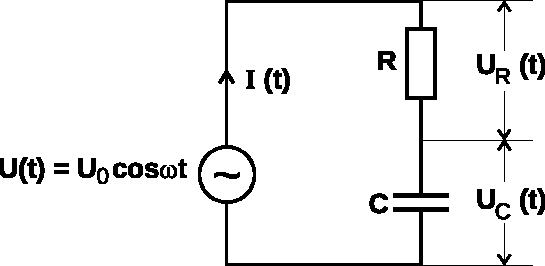
\includegraphics[width=0.5\textwidth]{build/Abb_2.pdf}
    \caption {Schematische Darstellung des Scans vom Augenmodell\cite{VUS1}.}
    \label{fig:Abb_2}
  \end{figure}
